\documentclass[a4paper]{article}

\usepackage[english]{babel}
\usepackage[utf8x]{inputenc}
\usepackage[T1]{fontenc}
\usepackage[a4paper,top=3cm,bottom=2cm,left=3cm,right=3cm,marginparwidth=1.75cm]{geometry}
\usepackage{graphicx}
\usepackage[colorlinks=true, allcolors=blue]{hyperref}

\title{Pick Up! SDSUI}
\author{Michael Chan (chanmic), Ryan Miura (miurary), \\Christopher Cooper (cooperchri), Jordan Clark (clarkj3), Ziyu Xiong (xiongz)}

\begin{document}
\maketitle

\section{User Interface Prototypes:}

\subsection{UI Prototype - User Authentication}
\includegraphics[width=\textwidth]{images/login-1}
If the user decides to click the "create" button to create an account to login, they will be redirected towards the account creation page.

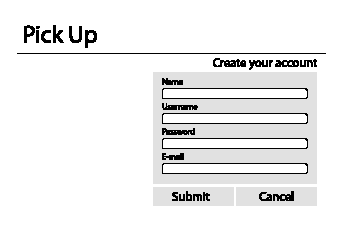
\includegraphics[width=\textwidth]{images/signup1.eps}
At this screen, the user is prompted for different fields. The user will need to fill out a name, username, password, and e-mail to be associated with the account. If all the fields are valid, the user will be able to click "submit" and create an account. In the case that a field is invalid or empty, they will be prompted with a pop-up indicating that they need to fill out all fields after clicking "submit". If the user chooses not to create an account, they can click the "cancel" button to return to the login page.

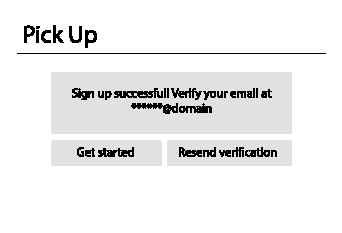
\includegraphics[width=\textwidth]{images/signup2.eps}
If the user clicks "submit" and has completed all the fields, they will be redirected to a "success" page. They will be required to verify their email in order to use all of the website. If they didn't verify their email, the user is limited in functions and will be redirected to this page when attempting functions for verified users. If they didn't receive an email, they can click "resend verification" to try again.

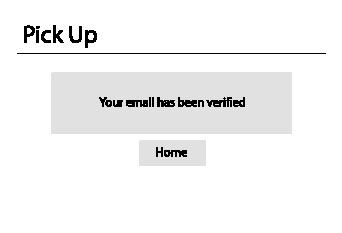
\includegraphics[width=\textwidth]{images/signup3.eps}
If the user successfully verifies their email, then the link in the email will redirect to this page, indicating that their account is ready for full use.

\subsection{UI Prototype - Search Events}

\includegraphics[width=\textwidth]{images/login-1}
The first screen users will come to is the login screen. In this screen, the user will enter the username associated with their account in the username field and their password in the pass field. The password will not be shown in the box and will instead show a dot or asterisk for each character. The user then clicks on the Submit button to log in. The system will then authenticate their user information and pass back a unique login ID for keeping them logged in while redirected. The system then redirects the user to their account homepage.

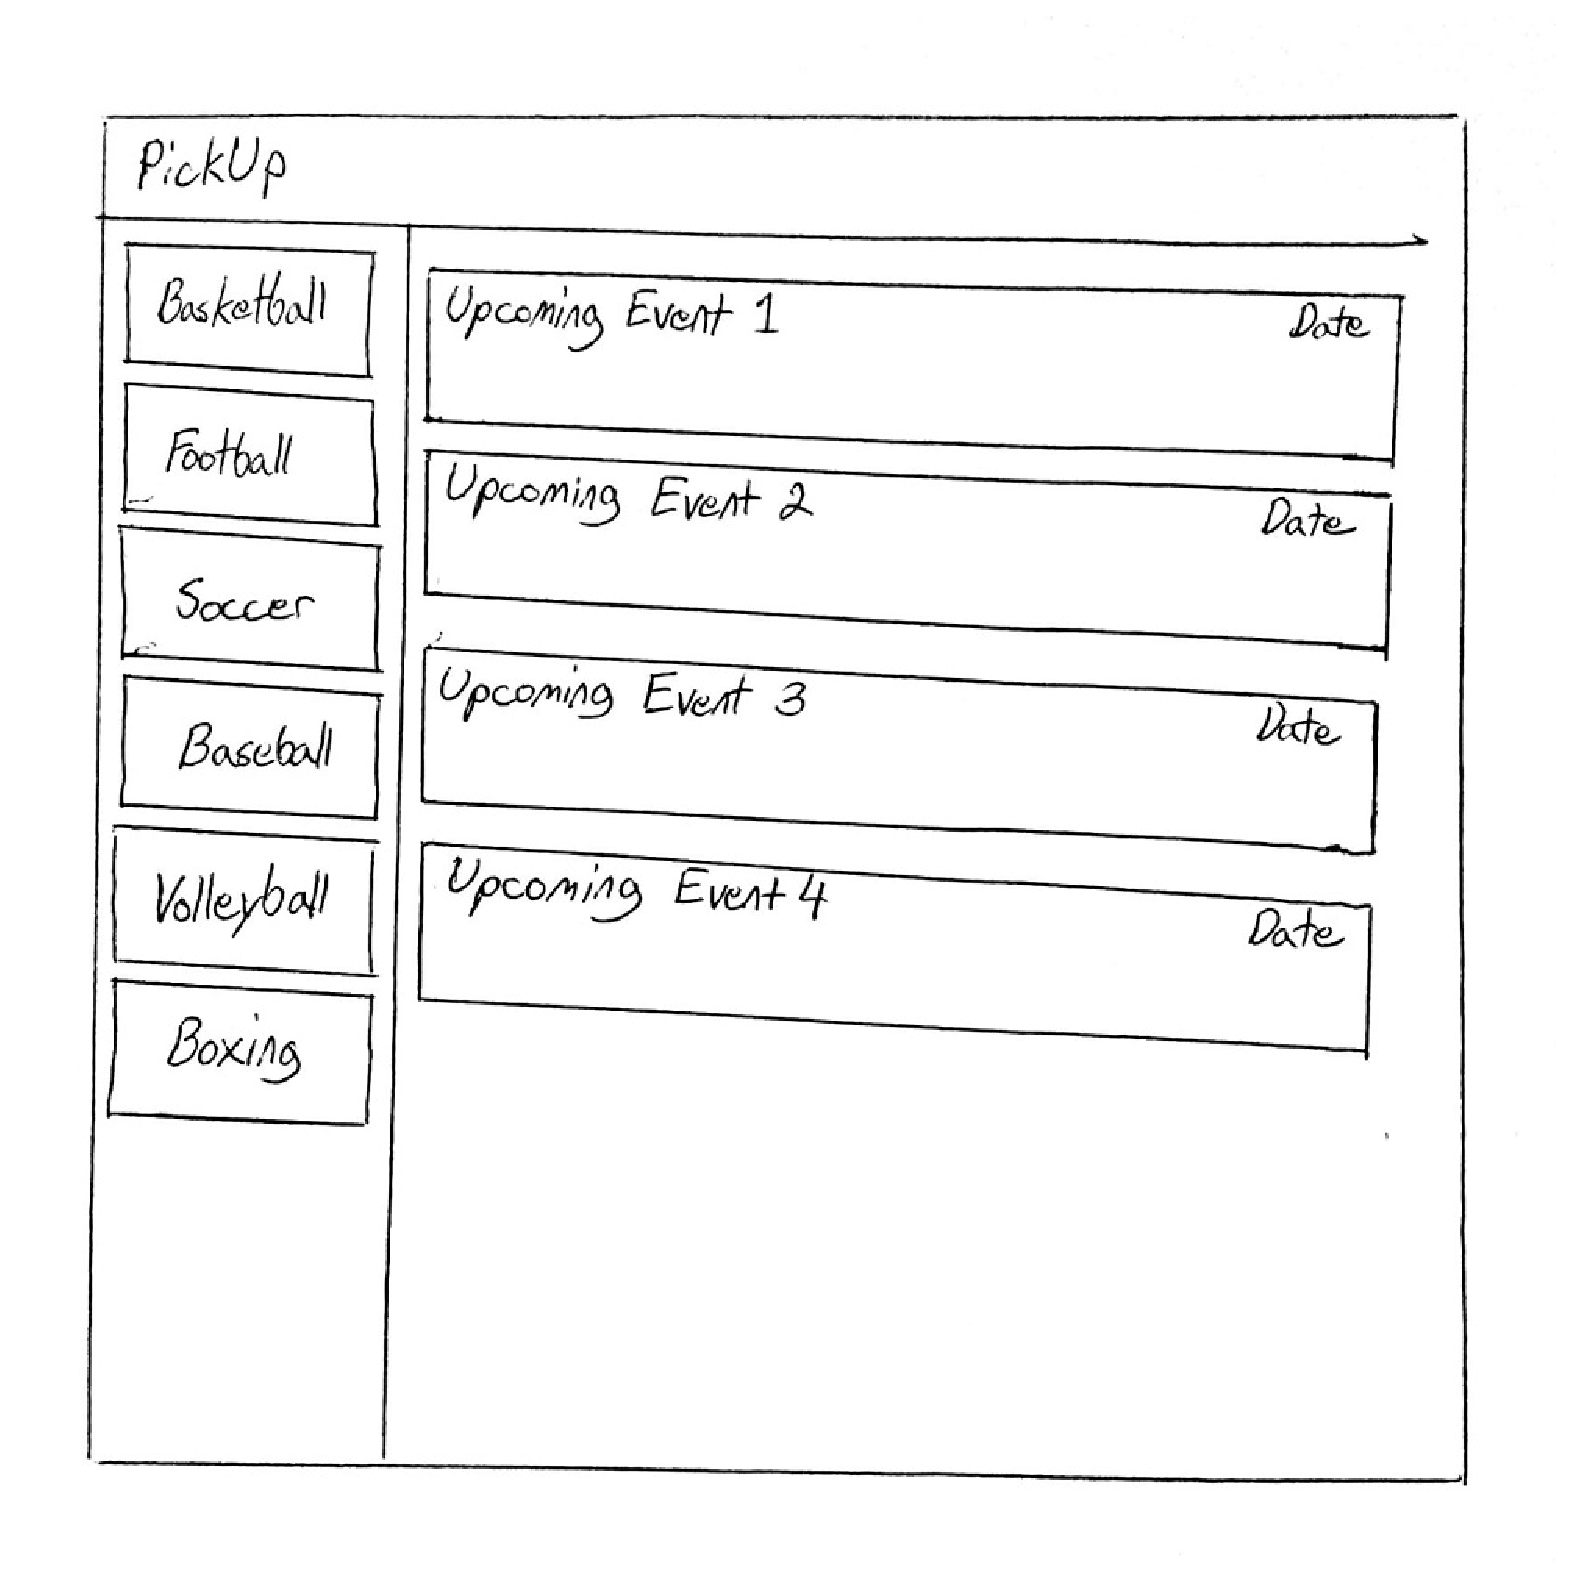
\includegraphics[width=\textwidth]{images/homepage-1}
This screen is the account homepage for the user. In order to start searching for new events to apply to, the user will select one of the sports in the sidebar to the left of the screen. This will redirect them to the specific sport's search results page.

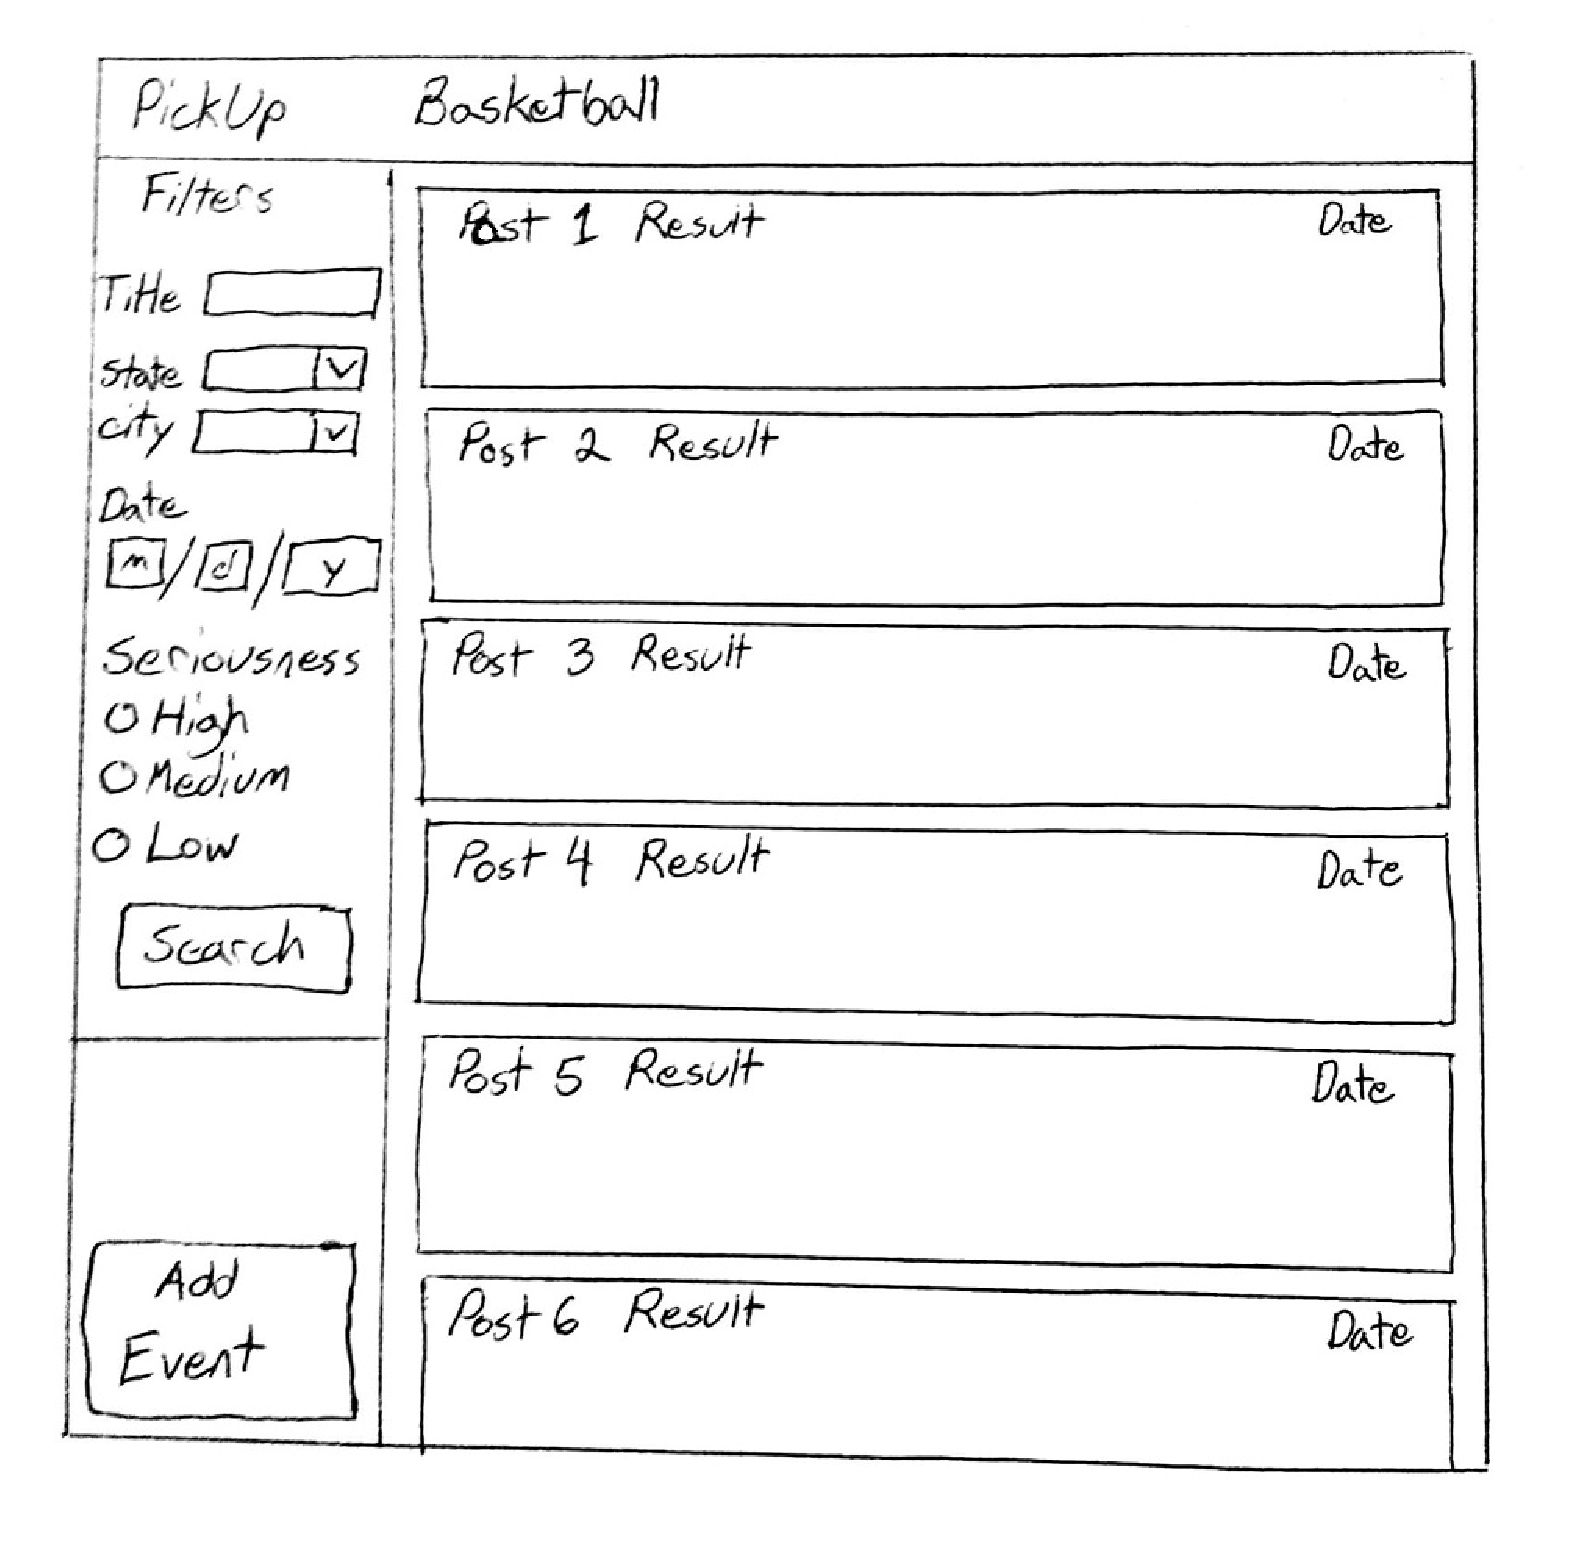
\includegraphics[width=\textwidth]{images/search-1}
The search results page for each individual sport has a sidebar of filters and a main section showing the results from the search. The filters can be used by entering data into the filter text boxes and then pressing the search button below the filter entry boxes. This is the end of the search event use case of the website and the user has successfully searched for new events to participate in.
\subsection{UI Prototype - Post Event}
After logging in the PickUp! Website, users choose the event category page that they wish to add to.
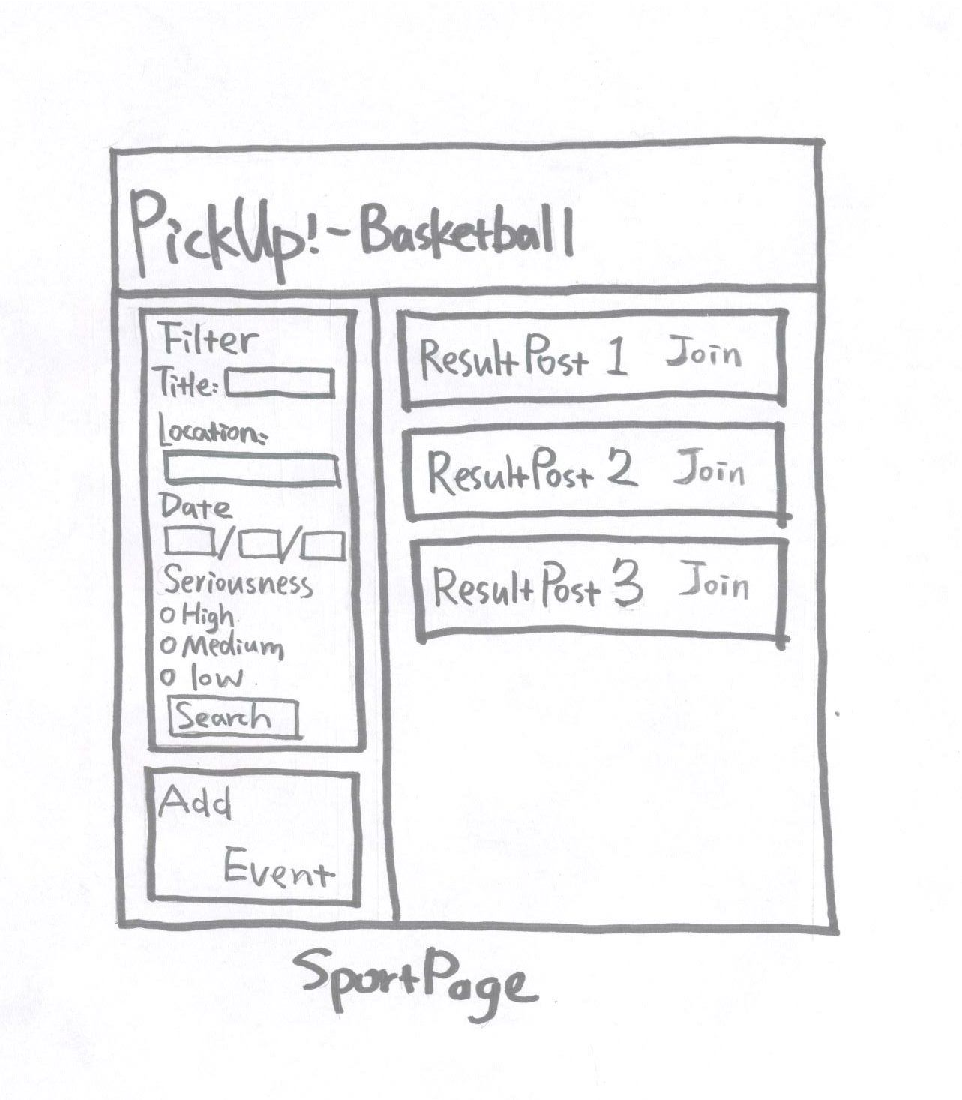
\includegraphics[width=\textwidth]{images/sport_page.pdf}
Taking basketball as an example of Sport Page, there is a button called “add event” under the filter. If the users click on that “add event” button, the user will be able to create a new event.

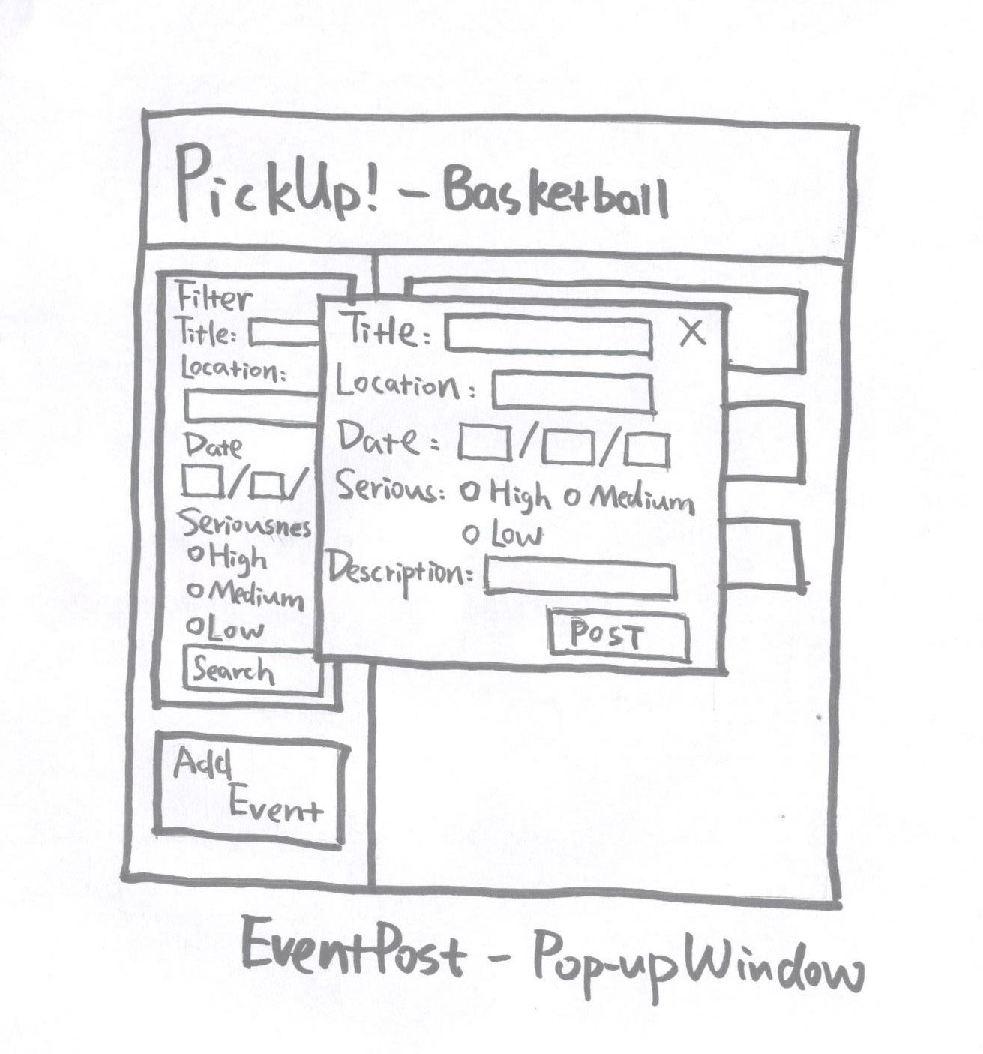
\includegraphics[width=\textwidth]{images/post_pop-up_window.pdf}
After clicking on the “Add Event” button, there will be a pop-up window at the middle of the screen asking users to fill out all the information about the event. If users miss some information in this window, the website will give an alert message, such as “You need to type in all the information about your event.” After filling all the blanks in the pop-up window, the user clicks on the “post” button to exit the pop-up window. All the information just added by user will be sent to database and sort by class or element id. 

\section{Class Diagrams}
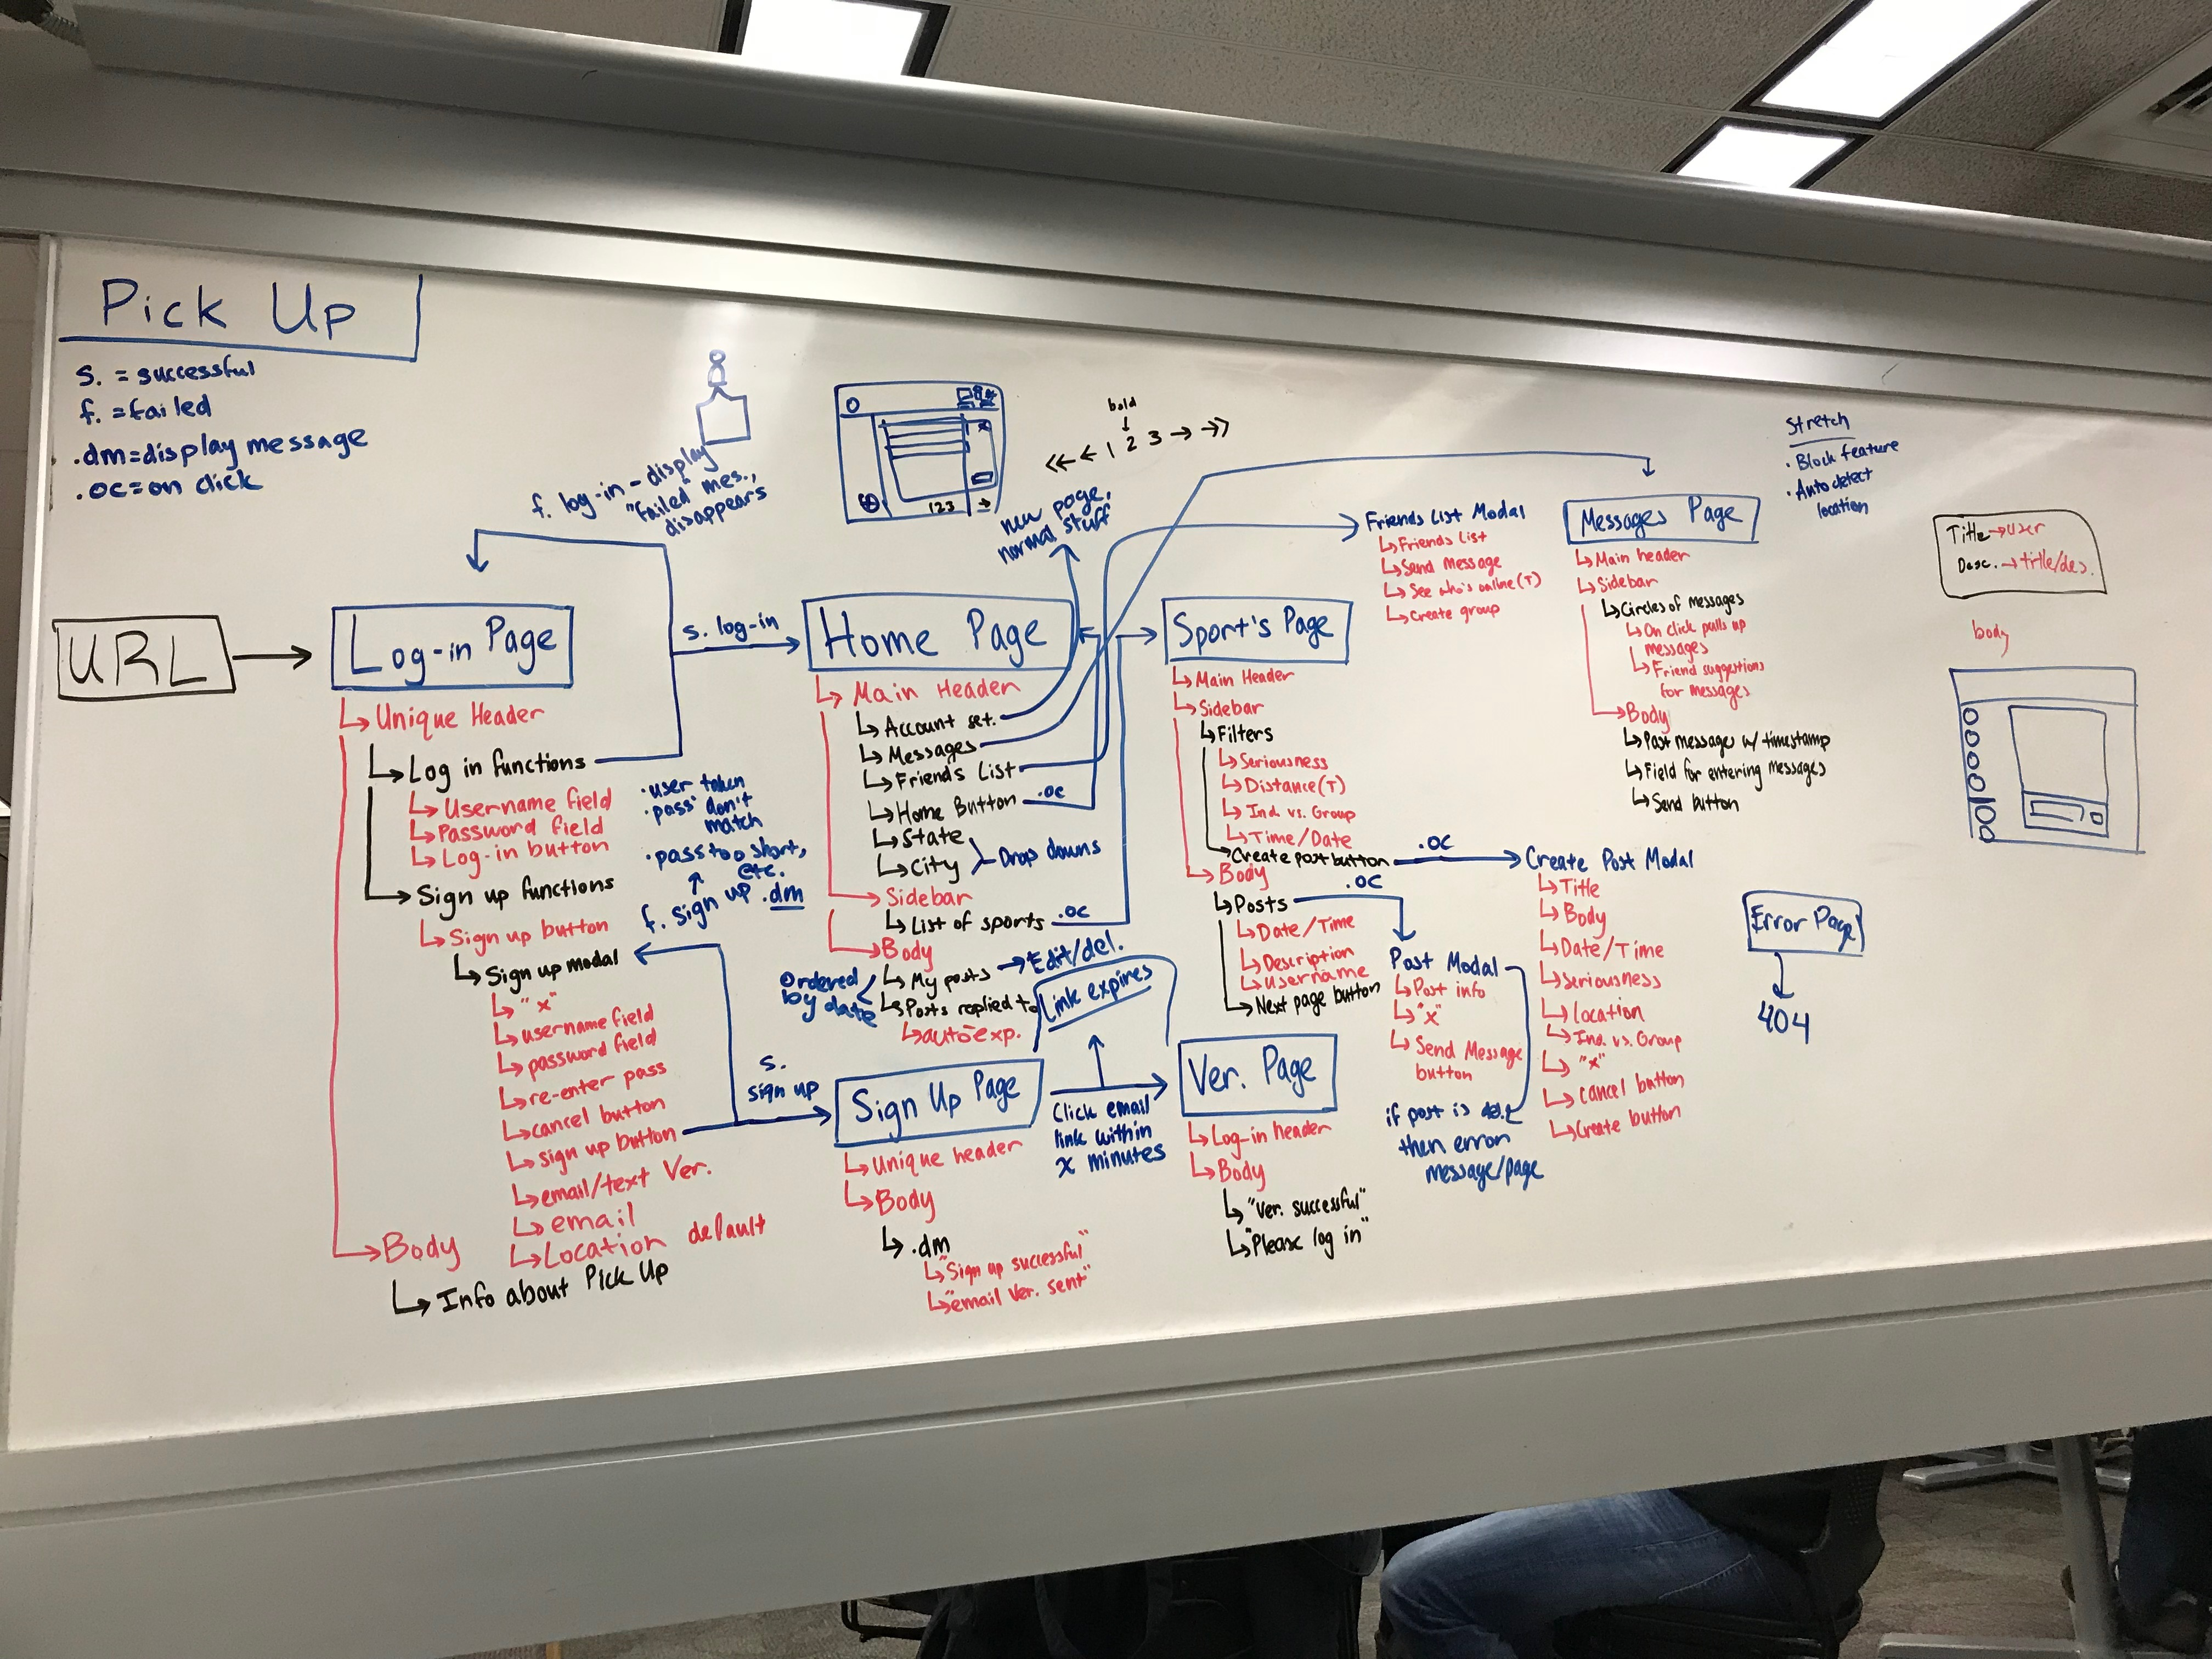
\includegraphics[width=\textwidth]{images/pic1.jpg}

\section{Sequence Diagrams}
\subsection{UML Sequence - User Authentication}
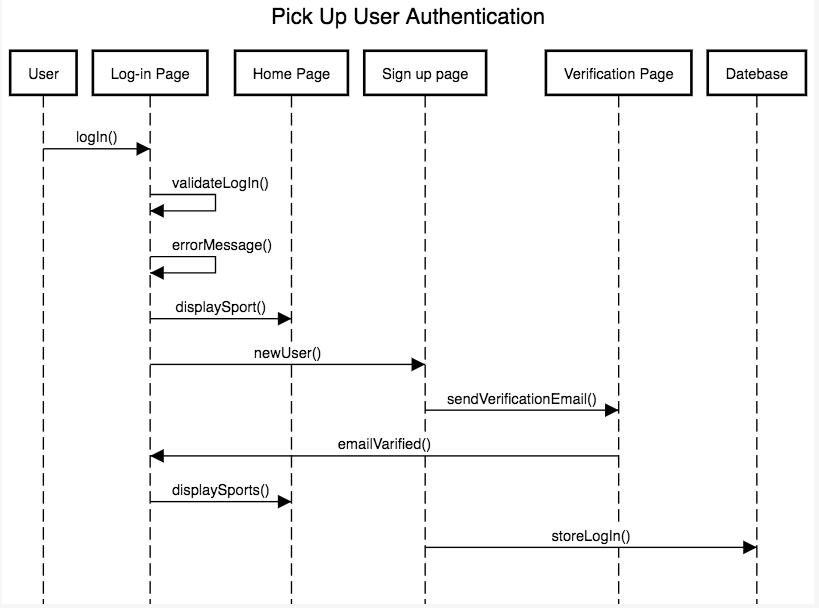
\includegraphics[width=\textwidth]{images/uml1.png}

\subsection{UML Sequence - Search Events}
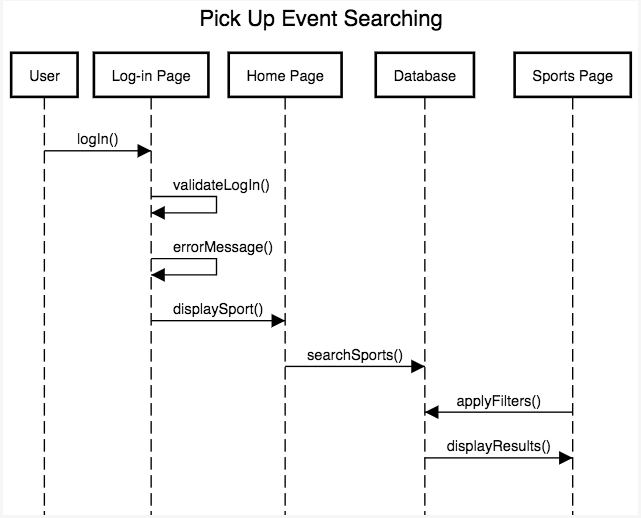
\includegraphics[width=\textwidth]{images/uml2.png}

\subsection{UML Sequence - Post Events}
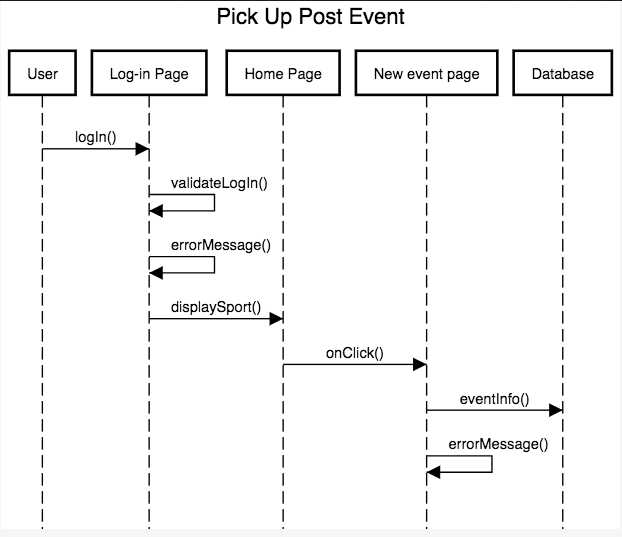
\includegraphics[width=\textwidth]{images/uml3.png}

\section{Meeting Report:}
This week we met in the library for a few hours. There, we flushed out the design of our website. We determined which functions would need completely new pages, how our pages would look, where buttons would be, and more. It was a great overview for the HTML we have to write. We didn’t go in depth with things regarding JS, but it should be pretty self-explanatory where JS is needed when reading the diagram. The client-side JS we would need also seems fairly simple to write, so we didn’t sweat over it much. After we finished the diagram, we assigned parts of Assignment 3 to each of our members and went our separate ways.

Through this next week, we are hoping to first and foremost finish Assignment 3. After that, I think we want to do a bit more design and build off of what we did this week. We all want to be on the same page before we start coding. If we get to a good point, we will start coding this week. I think we would all feel better about starting the code early to give us a larger time frame.

Michael, Chris, and Ziyu worked on the User Interface Prototypes. Jordan worked on the Sequence Diagrams. I worked on the Class Diagram and this Meeting Report.

We were able to meet with everyone this week.




\end{document}